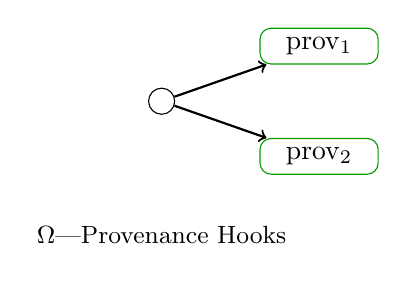
\begin{tikzpicture}[
    snap/.style={circle,draw=black,fill=white,minimum size=7pt},
    prov/.style={rectangle,draw=green!60!black,rounded corners,minimum width=1.5cm},
    arrow/.style={->, thick}
]

\node[snap] (S) at (0,0) {};

\node[prov] (P1) at (2,0.7) {prov$_1$};
\node[prov] (P2) at (2,-0.7) {prov$_2$};

\draw[arrow] (S)--(P1);
\draw[arrow] (S)--(P2);

\node at (0,-1.7) {\small $\Omega$---Provenance Hooks};

\end{tikzpicture}
